\documentclass[a4paper]{article}\usepackage[]{graphicx}\usepackage[]{color}
%% maxwidth is the original width if it is less than linewidth
%% otherwise use linewidth (to make sure the graphics do not exceed the margin)
\makeatletter
\def\maxwidth{ %
  \ifdim\Gin@nat@width>\linewidth
    \linewidth
  \else
    \Gin@nat@width
  \fi
}
\makeatother

\definecolor{fgcolor}{rgb}{0.345, 0.345, 0.345}
\newcommand{\hlnum}[1]{\textcolor[rgb]{0.686,0.059,0.569}{#1}}%
\newcommand{\hlstr}[1]{\textcolor[rgb]{0.192,0.494,0.8}{#1}}%
\newcommand{\hlcom}[1]{\textcolor[rgb]{0.678,0.584,0.686}{\textit{#1}}}%
\newcommand{\hlopt}[1]{\textcolor[rgb]{0,0,0}{#1}}%
\newcommand{\hlstd}[1]{\textcolor[rgb]{0.345,0.345,0.345}{#1}}%
\newcommand{\hlkwa}[1]{\textcolor[rgb]{0.161,0.373,0.58}{\textbf{#1}}}%
\newcommand{\hlkwb}[1]{\textcolor[rgb]{0.69,0.353,0.396}{#1}}%
\newcommand{\hlkwc}[1]{\textcolor[rgb]{0.333,0.667,0.333}{#1}}%
\newcommand{\hlkwd}[1]{\textcolor[rgb]{0.737,0.353,0.396}{\textbf{#1}}}%

\usepackage{framed}
\makeatletter
\newenvironment{kframe}{%
 \def\at@end@of@kframe{}%
 \ifinner\ifhmode%
  \def\at@end@of@kframe{\end{minipage}}%
  \begin{minipage}{\columnwidth}%
 \fi\fi%
 \def\FrameCommand##1{\hskip\@totalleftmargin \hskip-\fboxsep
 \colorbox{shadecolor}{##1}\hskip-\fboxsep
     % There is no \\@totalrightmargin, so:
     \hskip-\linewidth \hskip-\@totalleftmargin \hskip\columnwidth}%
 \MakeFramed {\advance\hsize-\width
   \@totalleftmargin\z@ \linewidth\hsize
   \@setminipage}}%
 {\par\unskip\endMakeFramed%
 \at@end@of@kframe}
\makeatother

\definecolor{shadecolor}{rgb}{.97, .97, .97}
\definecolor{messagecolor}{rgb}{0, 0, 0}
\definecolor{warningcolor}{rgb}{1, 0, 1}
\definecolor{errorcolor}{rgb}{1, 0, 0}
\newenvironment{knitrout}{}{} % an empty environment to be redefined in TeX

\usepackage{alltt}

\usepackage{amsmath}
\usepackage{amssymb}
\usepackage{parskip}
\usepackage{natbib}
\bibpunct{(}{)}{;}{a}{}{,}
\usepackage{hyperref}
\usepackage[margin=1in]{geometry}
\usepackage[labelfont={bf}, margin=0.5cm]{caption}

%\VignetteIndexEntry{ANOM}
%\VignetteEngine{knitr::knitr}

\title{Analysis of means: Examples using package \texttt{ANOM}}
\date{}
\author{Philip Pallmann}
\IfFileExists{upquote.sty}{\usepackage{upquote}}{}
\begin{document}

\maketitle

\tableofcontents

%%%%%%%%%%%%%%%%%%%%%%%%%%%%%%%%%%%%%%%%%%%%%%%%%%%%%%%%%%%%%%%%%%%%%%%%%%%%%%%%%%%%%%%%%%%%%%%%%%%%%%%%%%%%%%%%%%%%%%%%%%%%%%%%%%
%%%%%%%%%%%%%%%%%%%%%%%%%%%%%%%%%%%%%%%%%%%%%%%%%%%%%%%%%%%%%%%%%%%%%%%%%%%%%%%%%%%%%%%%%%%%%%%%%%%%%%%%%%%%%%%%%%%%%%%%%%%%%%%%%%
%%%%%%%%%%%%%%%%%%%%%%%%%%%%%%%%%%%%%%%%%%%%%%%%%%%%%%%%%%%%%%%%%%%%%%%%%%%%%%%%%%%%%%%%%%%%%%%%%%%%%%%%%%%%%%%%%%%%%%%%%%%%%%%%%%

\section{Introduction}

The analysis of means (ANOM) is a graphical method for presenting multiple group comparisons with an overall mean (``grand mean"). Ever since Ott published his pioneering paper \citep{Ott1967}, ANOM has enjoyed great popularity in quality control, and piles of extensions and applications have been discussed. A nice SAS-based overview of ANOM is given in the book by \citet{Nelson2005}.

The purpose of this vignette is to illustrate how R's broad functionality can be exploited for ANOM-type data analysis. We have already elaborated on various real-world data applications of ANOM in the tutorial publication accompanying this package \citep{Pallmann2015}. In the following we want to delve into some further non-trivial data scenarios:
\begin{itemize}
  \item ANOM with more than one factor e.g., in a two-way layout (Section \ref{Twoway}),
  \item ANOM with non-normal data e.g., (overdispersed) Poisson count data using generalized linear models (Section \ref{Count}),
  \item ANOM with correlated data in clustered, nested, hierarchical, or multilevel structures e.g., repeated measures with multiple raters using linear mixed-effects models (Section \ref{Mixed}).
\end{itemize}
All comparisons are performed at a familywise type I error level of 5\%. 



\clearpage

%%%%%%%%%%%%%%%%%%%%%%%%%%%%%%%%%%%%%%%%%%%%%%%%%%%%%%%%%%%%%%%%%%%%%%%%%%%%%%%%%%%%%%%%%%%%%%%%%%%%%%%%%%%%%%%%%%%%%%%%%%%%%%%%%%
%%%%%%%%%%%%%%%%%%%%%%%%%%%%%%%%%%%%%%%%%%%%%%%%%%%%%%%%%%%%%%%%%%%%%%%%%%%%%%%%%%%%%%%%%%%%%%%%%%%%%%%%%%%%%%%%%%%%%%%%%%%%%%%%%%
%%%%%%%%%%%%%%%%%%%%%%%%%%%%%%%%%%%%%%%%%%%%%%%%%%%%%%%%%%%%%%%%%%%%%%%%%%%%%%%%%%%%%%%%%%%%%%%%%%%%%%%%%%%%%%%%%%%%%%%%%%%%%%%%%%

\section{ANOM in a two-way layout}
\label{Twoway}

\citet{Nelson2005} describe a trial on 30 male cancer patients in a balanced complete two-way layout. Each patient was treated with one therapy (chemo or radiation) and one out of three drugs (named 1, 2, and 3), and the level of hemoglobin was measured afterwards.

\begin{knitrout}
\definecolor{shadecolor}{rgb}{0.969, 0.969, 0.969}\color{fgcolor}\begin{kframe}
\begin{alltt}
\hlkwd{library}\hlstd{(ANOM)}
\hlkwd{data}\hlstd{(hemoglobin)}
\end{alltt}
\end{kframe}
\end{knitrout}

The six drug-therapy combinations may be compared in a simplified pseudo-one-way layout where the new factor's levels are the combinations of therapy and drug.

\begin{knitrout}
\definecolor{shadecolor}{rgb}{0.969, 0.969, 0.969}\color{fgcolor}\begin{kframe}
\begin{alltt}
\hlstd{hemoglobin}\hlopt{$}\hlstd{the} \hlkwb{<-} \hlkwd{as.factor}\hlstd{(}\hlkwd{abbreviate}\hlstd{(hemoglobin}\hlopt{$}\hlstd{therapy))}
\hlstd{hemoglobin}\hlopt{$}\hlstd{td} \hlkwb{<-} \hlkwd{with}\hlstd{(hemoglobin, the}\hlopt{:}\hlstd{drug)}
\hlstd{hemodel} \hlkwb{<-} \hlkwd{lm}\hlstd{(level} \hlopt{~} \hlstd{td, hemoglobin)}
\hlstd{he} \hlkwb{<-} \hlkwd{glht}\hlstd{(hemodel,} \hlkwd{mcp}\hlstd{(}\hlkwc{td}\hlstd{=}\hlstr{"GrandMean"}\hlstd{),} \hlkwc{alternative}\hlstd{=}\hlstr{"two.sided"}\hlstd{)}
\hlkwd{ANOM}\hlstd{(he,} \hlkwc{xlabel}\hlstd{=}\hlstr{"Treatment"}\hlstd{,} \hlkwc{ylabel}\hlstd{=}\hlstr{"Hemoglobin Level"}\hlstd{)}
\end{alltt}
\end{kframe}\begin{figure}
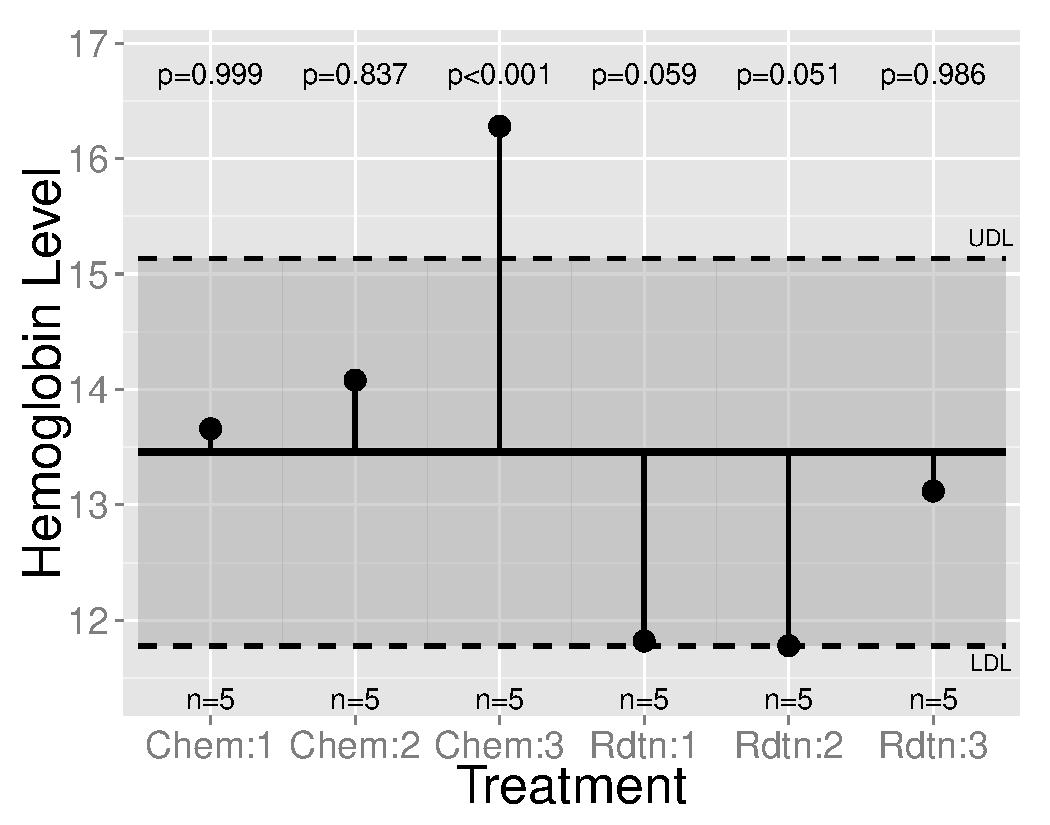
\includegraphics[width=\maxwidth]{figure/PSEUDOONEWAY-1} \caption[ANOM decision chart for the hemoglobin data based one a pseudo-one-way analysis]{ANOM decision chart for the hemoglobin data based one a pseudo-one-way analysis.}\label{fig:PSEUDOONEWAY}
\end{figure}


\end{knitrout}

We find that chemotherapy together with drug 3 leads to hemoglobin levels that are significantly above the grand mean (Figure 1). On the contrary, if radiation therapy is combined with either drug 1 or 2, the levels of hemoglobin are very close to the lower decision limit.

Acting on the assumption that the two treatment factors ``therapy" and ``drug" do not interact, we may also investigate the marginal drug effects across both therapies. An analysis of variance suggests that the interaction effect is negligible.

\begin{knitrout}
\definecolor{shadecolor}{rgb}{0.969, 0.969, 0.969}\color{fgcolor}\begin{kframe}
\begin{alltt}
\hlstd{hemodel2} \hlkwb{<-} \hlkwd{lm}\hlstd{(level} \hlopt{~} \hlstd{drug} \hlopt{*} \hlstd{therapy, hemoglobin)}
\hlkwd{anova}\hlstd{(hemodel2)}
\end{alltt}
\begin{verbatim}
## Analysis of Variance Table
## 
## Response: level
##              Df Sum Sq Mean Sq F value    Pr(>F)    
## drug          2 23.369  11.684  5.5385 0.0105262 *  
## therapy       1 44.408  44.408 21.0499 0.0001184 ***
## drug:therapy  2  2.245   1.122  0.5320 0.5941993    
## Residuals    24 50.632   2.110                      
## ---
## Signif. codes:  0 '***' 0.001 '**' 0.01 '*' 0.05 '.' 0.1 ' ' 1
\end{verbatim}
\end{kframe}
\end{knitrout}

This result clears the way for making reasonable inferences for drugs pooled over both types of therapy.

\begin{knitrout}
\definecolor{shadecolor}{rgb}{0.969, 0.969, 0.969}\color{fgcolor}\begin{kframe}
\begin{alltt}
\hlstd{hemodel3} \hlkwb{<-} \hlkwd{lm}\hlstd{(level} \hlopt{~} \hlstd{drug} \hlopt{+} \hlstd{therapy, hemoglobin)}
\hlstd{he3} \hlkwb{<-} \hlkwd{glht}\hlstd{(hemodel3,} \hlkwd{mcp}\hlstd{(}\hlkwc{drug}\hlstd{=}\hlstr{"GrandMean"}\hlstd{),} \hlkwc{alternative}\hlstd{=}\hlstr{"two.sided"}\hlstd{)}
\hlkwd{ANOM}\hlstd{(he3,} \hlkwc{xlabel}\hlstd{=}\hlstr{"Drug"}\hlstd{,} \hlkwc{ylabel}\hlstd{=}\hlstr{"Hemoglobin Level"}\hlstd{)}
\end{alltt}
\end{kframe}\begin{figure}
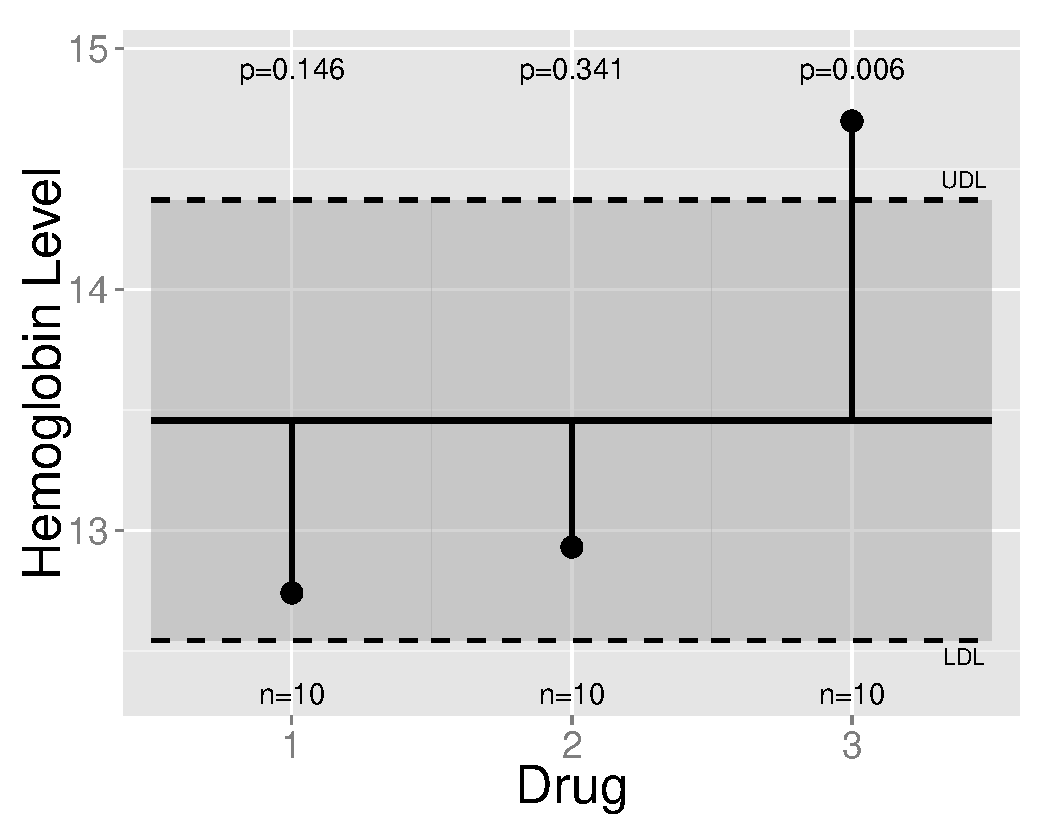
\includegraphics[width=\maxwidth]{figure/TWOWAY-1} \caption[ANOM decision chart for the hemoglobin data based on a two-way analysis]{ANOM decision chart for the hemoglobin data based on a two-way analysis.}\label{fig:TWOWAY}
\end{figure}


\end{knitrout}

Figure 2 shows that drug 3 raises hemoglobin levels significantly compared to the grand mean. Keep in mind that this type of pooled analysis would be inept in the presence of a therapy-drug interaction; here one should rather perform separate drug comparisons for radiation and for chemotherapy.

\clearpage

%%%%%%%%%%%%%%%%%%%%%%%%%%%%%%%%%%%%%%%%%%%%%%%%%%%%%%%%%%%%%%%%%%%%%%%%%%%%%%%%%%%%%%%%%%%%%%%%%%%%%%%%%%%%%%%%%%%%%%%%%%%%%%%%%%
%%%%%%%%%%%%%%%%%%%%%%%%%%%%%%%%%%%%%%%%%%%%%%%%%%%%%%%%%%%%%%%%%%%%%%%%%%%%%%%%%%%%%%%%%%%%%%%%%%%%%%%%%%%%%%%%%%%%%%%%%%%%%%%%%%
%%%%%%%%%%%%%%%%%%%%%%%%%%%%%%%%%%%%%%%%%%%%%%%%%%%%%%%%%%%%%%%%%%%%%%%%%%%%%%%%%%%%%%%%%%%%%%%%%%%%%%%%%%%%%%%%%%%%%%%%%%%%%%%%%%

\section{ANOM with (overdispersed) count data}
\label{Count}

\citet{Beall1942} reports a study on the effectiveness of six insect sprays to control the tomato hornworm \textit{Manduca quinquemaculata} (formerly called \textit{Phlegethontius quinquemaculatus}), which is a common pest of solanaceae. The experiment was carried out in a randomized complete block design: each spray was applied to plants in each of six blocks, and the number of insects found after treatment was counted and recorded (taking two random samples per block and spray).

The data is stored in R's basic \texttt{datasets} package, but this version is incomplete as the block structure of the experiment was missed out for some reason. We include a block variable according to Table 7 in Beall's original publication.

\begin{knitrout}
\definecolor{shadecolor}{rgb}{0.969, 0.969, 0.969}\color{fgcolor}\begin{kframe}
\begin{alltt}
\hlkwd{data}\hlstd{(InsectSprays)}
\hlstd{InsectSprays}\hlopt{$}\hlstd{block} \hlkwb{<-} \hlkwd{as.factor}\hlstd{(}\hlkwd{rep}\hlstd{(}\hlnum{1}\hlopt{:}\hlnum{6}\hlstd{,} \hlkwc{each}\hlstd{=}\hlnum{2}\hlstd{))}
\end{alltt}
\end{kframe}
\end{knitrout}

A common distributional assumption for count data is Poisson, so it sounds like a good idea to fit a Poisson generalized linear model with a logarithmic link function to the data. However, recall that the variance of a Poisson random variable equals its expected value. This basic assumption is more often than not violated with real-world data, and we usually include a variance inflation factor $\phi$ in the model to cope with this overdispersion (or extra-Poisson variability).

\begin{knitrout}
\definecolor{shadecolor}{rgb}{0.969, 0.969, 0.969}\color{fgcolor}\begin{kframe}
\begin{alltt}
\hlstd{insmodel1} \hlkwb{<-} \hlkwd{glm}\hlstd{(count} \hlopt{~} \hlstd{spray} \hlopt{+} \hlstd{block,} \hlkwc{data}\hlstd{=InsectSprays,}
                 \hlkwc{family}\hlstd{=}\hlkwd{quasipoisson}\hlstd{(}\hlkwc{link}\hlstd{=}\hlstr{"log"}\hlstd{))}
\hlkwd{summary}\hlstd{(insmodel1)}\hlopt{$}\hlstd{dispersion}
\end{alltt}
\begin{verbatim}
## [1] 1.198022
\end{verbatim}
\end{kframe}
\end{knitrout}

In our case the estimated variance inflation of 19.8\% is negligible, hence we will most likely not harm our analysis when using a simple Poisson GLM without an overdispersion parameter. An analysis of deviance reveals that both treatment and block bring about highly significant effects.

\begin{knitrout}
\definecolor{shadecolor}{rgb}{0.969, 0.969, 0.969}\color{fgcolor}\begin{kframe}
\begin{alltt}
\hlstd{insmodel2} \hlkwb{<-} \hlkwd{glm}\hlstd{(count} \hlopt{~} \hlstd{spray} \hlopt{+} \hlstd{block,} \hlkwc{data}\hlstd{=InsectSprays,}
                 \hlkwc{family}\hlstd{=}\hlkwd{poisson}\hlstd{(}\hlkwc{link}\hlstd{=}\hlstr{"log"}\hlstd{))}
\hlkwd{anova}\hlstd{(insmodel2,} \hlkwc{test}\hlstd{=}\hlstr{"Chisq"}\hlstd{)}
\end{alltt}
\begin{verbatim}
## Analysis of Deviance Table
## 
## Model: poisson, link: log
## 
## Response: count
## 
## Terms added sequentially (first to last)
## 
## 
##       Df Deviance Resid. Df Resid. Dev  Pr(>Chi)    
## NULL                     71     409.04              
## spray  5   310.71        66      98.33 < 2.2e-16 ***
## block  5    25.34        61      72.99 0.0001198 ***
## ---
## Signif. codes:  0 '***' 0.001 '**' 0.01 '*' 0.05 '.' 0.1 ' ' 1
\end{verbatim}
\end{kframe}
\end{knitrout}

We perform an ANOM to find out which insect sprays lead to lower or higher counts of insects compared to average. The logarithmic transformation of the counts is automatically reversed to simplify interpretation of the resulting graph. 

\begin{knitrout}
\definecolor{shadecolor}{rgb}{0.969, 0.969, 0.969}\color{fgcolor}\begin{kframe}
\begin{alltt}
\hlstd{ins} \hlkwb{<-} \hlkwd{glht}\hlstd{(insmodel2,} \hlkwd{mcp}\hlstd{(}\hlkwc{spray}\hlstd{=}\hlstr{"GrandMean"}\hlstd{))}
\hlkwd{ANOM}\hlstd{(ins)}
\end{alltt}
\end{kframe}\begin{figure}
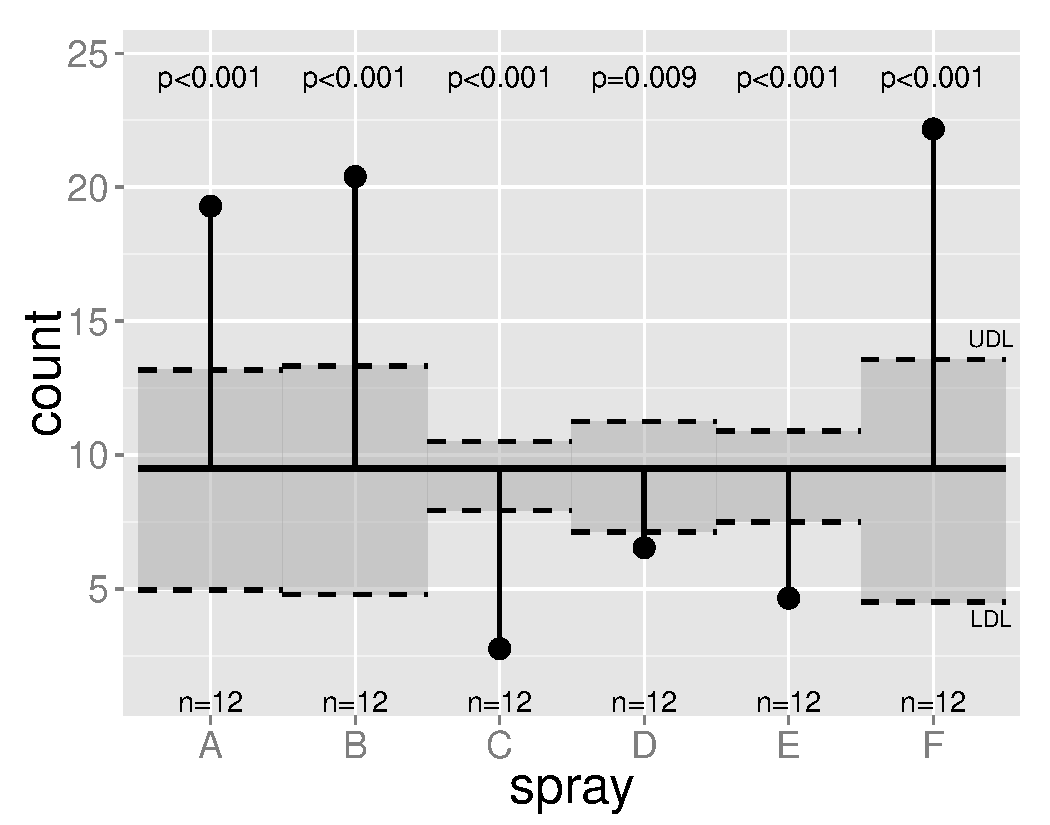
\includegraphics[width=\maxwidth]{figure/INSECTS2a-1} \caption[ANOM decision chart for the insect spray data based on a Poisson GLM]{ANOM decision chart for the insect spray data based on a Poisson GLM.}\label{fig:INSECTS2a}
\end{figure}


\end{knitrout}

Figure 3 shows that all six treatments are significantly different from the grand mean: more insects were counted after applying sprays A, B, and F, and fewer with sprays C through E. The varying widths of the gray band (upped minus lower decision limit) just reflect the dependence of the Poisson variance on the expected value.

\clearpage

%%%%%%%%%%%%%%%%%%%%%%%%%%%%%%%%%%%%%%%%%%%%%%%%%%%%%%%%%%%%%%%%%%%%%%%%%%%%%%%%%%%%%%%%%%%%%%%%%%%%%%%%%%%%%%%%%%%%%%%%%%%%%%%%%%
%%%%%%%%%%%%%%%%%%%%%%%%%%%%%%%%%%%%%%%%%%%%%%%%%%%%%%%%%%%%%%%%%%%%%%%%%%%%%%%%%%%%%%%%%%%%%%%%%%%%%%%%%%%%%%%%%%%%%%%%%%%%%%%%%%
%%%%%%%%%%%%%%%%%%%%%%%%%%%%%%%%%%%%%%%%%%%%%%%%%%%%%%%%%%%%%%%%%%%%%%%%%%%%%%%%%%%%%%%%%%%%%%%%%%%%%%%%%%%%%%%%%%%%%%%%%%%%%%%%%%

\section{ANOM with linear mixed-effects models}
\label{Mixed}

\citet{Pinheiro2000} describe data from an investigation of ergonomic stools performed by \citet{Wretenberg1993}. They had nine people assess the physical effort to rise from each of four stool types: a stool of ordinary height, a low ordinary stool, a one-legged stool, and a pneumatic stool. Each subject tested each stool type once and rated the perceived exertion on the so-called Borg scale, which takes values from 6 to 20. We wish to detect types of stools that are significantly more or less difficult to rise from in comparison to average.

\begin{knitrout}
\definecolor{shadecolor}{rgb}{0.969, 0.969, 0.969}\color{fgcolor}\begin{kframe}
\begin{alltt}
\hlkwd{library}\hlstd{(nlme)}
\hlkwd{data}\hlstd{(ergoStool)}
\end{alltt}
\end{kframe}
\end{knitrout}

This is a complete block design; each of the four stools under study is evaluated nine times. One challenge is that the scoring is clearly subjective e.g., a person suffering from chronic back pain is more likely to assign lower ratings than a healthy individual. To account for this variability between raters, a linear mixed-effects model is our method of choice.

The model for the $i$th individual has the general form
\begin{equation*}
\mathbf{y}_i = \mathbf{X}_i \boldsymbol{\beta} + \mathbf{Z}_i \mathbf{b}_i + \boldsymbol{\epsilon}_i
\end{equation*}
where $\mathbf{y}_i$ are the outcomes, $\boldsymbol{\beta}$ the fixed and $\mathbf{b}_i$ the random effects, $\mathbf{X}_i$ and $\mathbf{Z}_i$ the design matrices for the fixed and random effects, and $\boldsymbol{\epsilon}_i$ the residuals. We assume that $\mathbf{b}_i \sim \mathcal{N}(\mathbf{0}, \mathbf{D})$ and $\mathbf{e}_i \sim \mathcal{N}(\mathbf{0}, \mathbf{R}_i)$, and additionally $\operatorname{cov}(\mathbf{b}_i, \mathbf{e}_i) = \mathbf{0}$.

In our ergonomic stools example, we model fixed stool effects and treat the test persons as random. We hereby make the assumption that the testers are representative of all people who could sit on these stools and that their scorings are normally distributed with between-rater variance $\sigma_b$.

There are several concurrent and (in part) complementary frameworks for mixed-effects modeling which coexist in the R world. Here we illustrate ANOM using two of the most popular and best-established packages, \texttt{nlme} \citep{Pinheiro2013} and \texttt{lme4} \citep{Bates2013}.

\subsection{Using \texttt{nlme}}

We model the perceived effort to rise (on the Borg scale) as a function of the type of stool and include a random subject effect to acknowledge between-rater variability.

\begin{knitrout}
\definecolor{shadecolor}{rgb}{0.969, 0.969, 0.969}\color{fgcolor}\begin{kframe}
\begin{alltt}
\hlkwd{library}\hlstd{(nlme)}
\hlstd{esmodel1} \hlkwb{<-} \hlkwd{lme}\hlstd{(effort} \hlopt{~} \hlstd{Type,} \hlkwc{random}\hlstd{=}\hlopt{~}\hlnum{1}\hlopt{|}\hlstd{Subject,} \hlkwc{data}\hlstd{=ergoStool)}
\hlstd{es1} \hlkwb{<-} \hlkwd{glht}\hlstd{(esmodel1,} \hlkwd{mcp}\hlstd{(}\hlkwc{Type}\hlstd{=}\hlstr{"GrandMean"}\hlstd{),} \hlkwc{alternative}\hlstd{=}\hlstr{"two.sided"}\hlstd{)}
\hlkwd{ANOM}\hlstd{(es1,} \hlkwc{xlabel}\hlstd{=}\hlstr{"Stool Type"}\hlstd{,} \hlkwc{ylabel}\hlstd{=}\hlstr{"Exertion (Borg Scale)"}\hlstd{)}
\end{alltt}
\end{kframe}\begin{figure}
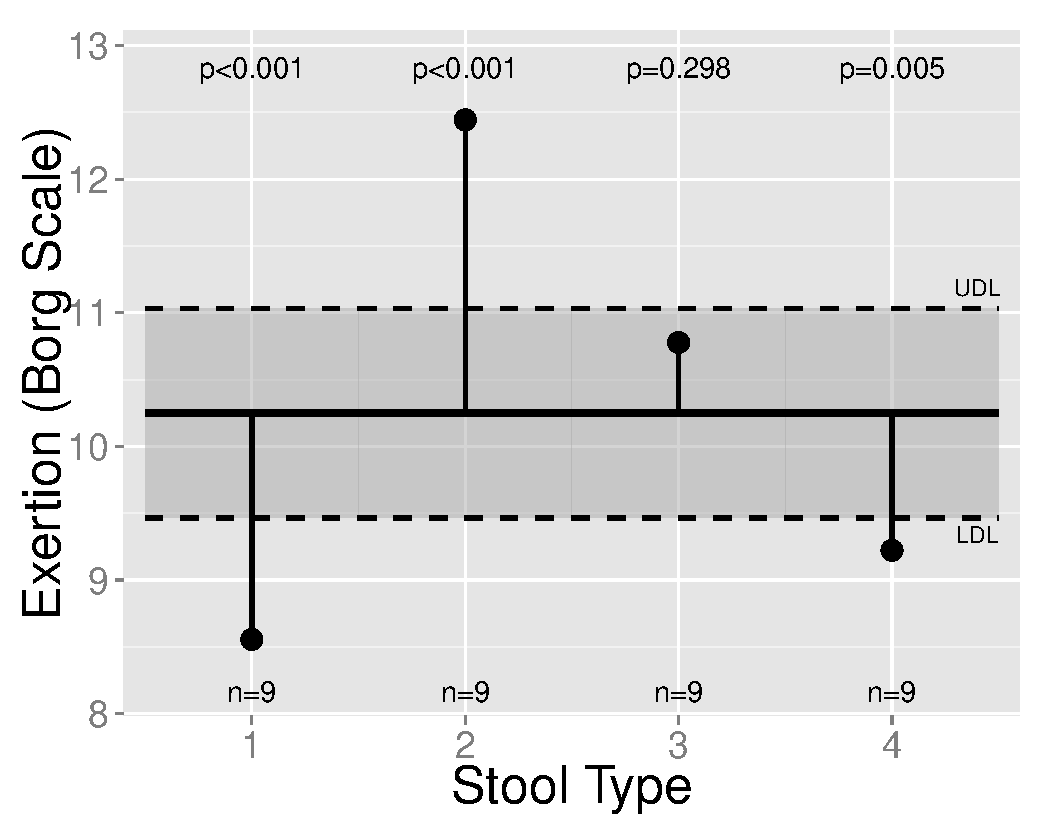
\includegraphics[width=\maxwidth]{figure/NLME-1} \caption[ANOM decision chart for the ergonomic stool data based on a linear mixed-effects model]{ANOM decision chart for the ergonomic stool data based on a linear mixed-effects model.}\label{fig:NLME}
\end{figure}


\end{knitrout}

Figure 4 displays that it is significantly more difficult to rise from stools of type 2. On the contrary, the perceived exertion is significantly below the grand mean for stool types 1 and 4.

\subsection{Using \texttt{lme4}}

An identical graphic can be generated with the functionality in \texttt{lme4}.

\begin{knitrout}
\definecolor{shadecolor}{rgb}{0.969, 0.969, 0.969}\color{fgcolor}\begin{kframe}
\begin{alltt}
\hlkwd{library}\hlstd{(lme4)}
\hlstd{esmodel2} \hlkwb{<-} \hlkwd{lmer}\hlstd{(effort} \hlopt{~} \hlstd{Type} \hlopt{+} \hlstd{(}\hlnum{1}\hlopt{|}\hlstd{Subject),} \hlkwc{data}\hlstd{=ergoStool)}
\hlstd{es2} \hlkwb{<-} \hlkwd{glht}\hlstd{(esmodel2,} \hlkwd{mcp}\hlstd{(}\hlkwc{Type}\hlstd{=}\hlstr{"GrandMean"}\hlstd{),} \hlkwc{alternative}\hlstd{=}\hlstr{"two.sided"}\hlstd{)}
\hlkwd{ANOM}\hlstd{(es2,} \hlkwc{xlabel}\hlstd{=}\hlstr{"Stool Type"}\hlstd{,} \hlkwc{ylabel}\hlstd{=}\hlstr{"Exertion (Borg Scale)"}\hlstd{)}
\end{alltt}
\end{kframe}
\end{knitrout}

Note that there are instances when the two mixed-effects model packages cannot be used interchangeably. Only \texttt{nlme} supports imposing a pattern like compound symmetry or AR(1) on the covariance matrix of the random effects and/or residuals whereas \texttt{lme4}'s strong points are sophisticated random effects hierarchies and nested structures, and it also fits generalized linear mixed-effects models.

\subsection{Ignoring the repeated structure}

One may wonder what would happen if we did not account for the fact that each chair was tested by several individuals. We fit a simple linear model and observe that the decision limits drift apart so that stool type 4 is no longer significant (Figure 5).

\begin{knitrout}
\definecolor{shadecolor}{rgb}{0.969, 0.969, 0.969}\color{fgcolor}\begin{kframe}
\begin{alltt}
\hlstd{esmodel3} \hlkwb{<-} \hlkwd{lm}\hlstd{(effort} \hlopt{~} \hlstd{Type, ergoStool)}
\hlstd{es3} \hlkwb{<-} \hlkwd{glht}\hlstd{(esmodel3,} \hlkwd{mcp}\hlstd{(}\hlkwc{Type}\hlstd{=}\hlstr{"GrandMean"}\hlstd{),} \hlkwc{alternative}\hlstd{=}\hlstr{"two.sided"}\hlstd{)}
\hlkwd{ANOM}\hlstd{(es3,} \hlkwc{xlabel}\hlstd{=}\hlstr{"Stool Type"}\hlstd{,} \hlkwc{ylabel}\hlstd{=}\hlstr{"Exertion (Borg Scale)"}\hlstd{)}
\end{alltt}
\end{kframe}\begin{figure}
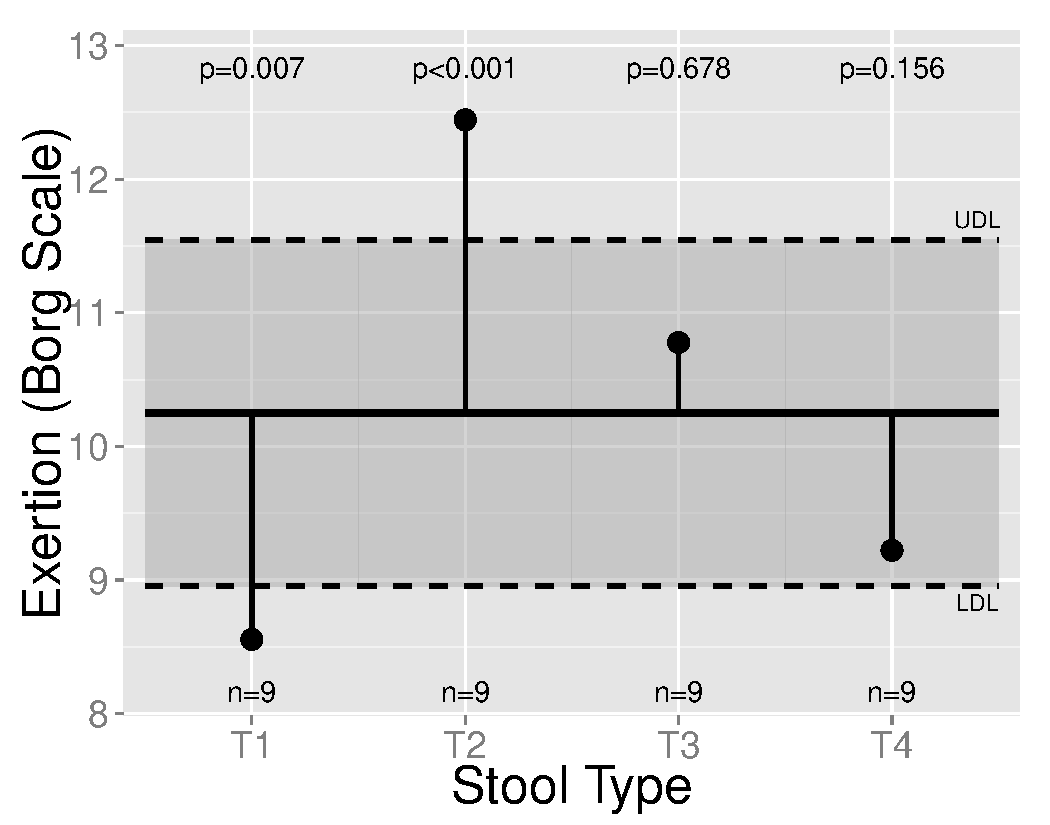
\includegraphics[width=\maxwidth]{figure/MIXIGNORE-1} \caption[ANOM decision chart for the ergonomic stool data based on a standard linear model]{ANOM decision chart for the ergonomic stool data based on a standard linear model.}\label{fig:MIXIGNORE}
\end{figure}


\end{knitrout}

The reason is quite simple: when fitting a mixed-effects model, we partition the total variance of the data into a component explained by the variability among the nine raters and a residual component. If we ignore the clustered structure of the data and fit a standard linear model, all variability is summed up in the residual variance, thus making it harder to detect significant stool effects.

\clearpage

%%%%%%%%%%%%%%%%%%%%%%%%%%%%%%%%%%%%%%%%%%%%%%%%%%%%%%%%%%%%%%%%%%%%%%%%%%%%%%%%%%%%%%%%%%%%%%%%%%%%%%%%%%%%%%%%%%%%%%%%%%%%%%%%%%
%%%%%%%%%%%%%%%%%%%%%%%%%%%%%%%%%%%%%%%%%%%%%%%%%%%%%%%%%%%%%%%%%%%%%%%%%%%%%%%%%%%%%%%%%%%%%%%%%%%%%%%%%%%%%%%%%%%%%%%%%%%%%%%%%%
%%%%%%%%%%%%%%%%%%%%%%%%%%%%%%%%%%%%%%%%%%%%%%%%%%%%%%%%%%%%%%%%%%%%%%%%%%%%%%%%%%%%%%%%%%%%%%%%%%%%%%%%%%%%%%%%%%%%%%%%%%%%%%%%%%

\bibliographystyle{abbrvnat}
\bibliography{vign}

\end{document}
